\hypertarget{sec-fairness}{%
\chapter{Algorithmic Fairness}\label{sec-fairness}}

\vspace{-15mm}\addtocontents{toc}{\textit{Florian Pfisterer}}

\textbf{Florian Pfisterer} \newline 
\emph{Ludwig-Maximilians-Universität München} \newline \newline 

In this chapter, we will explore algorithmic
fairness\index{algorithmic fairness}\index{fairness|see{algorithmic fairness}}
in automated decision-making and how we can build fair and unbiased (or
at least less biased) predictive models. Methods to help audit and
resolve bias in
\href{https://mlr3.mlr-org.com}{\texttt{mlr3}}\index{\texttt{mlr3}}
models are implemented in
\href{https://mlr3fairness.mlr-org.com}{\texttt{mlr3fairness}}\index{\texttt{mlr3fairness}}.
We will begin by first discussing some of the theory behind algorithmic
fairness and then show how this is implemented in \texttt{mlr3fairness}.

Automated decision-making systems based on data-driven models are
becoming increasingly common but without proper auditing, these models
may result in negative consequences for individuals, especially those
from underprivileged groups. The proliferation of such systems in
everyday life has made it important to address the potential for biases
in these models. As a real-world example, historical and sampling biases
have led to better quality medical data for patients from White ethnic
groups when compared with other ethnic groups. If a model is trained
primarily on data from White patients, then the model may appear `good'
with respect to a given performance metric (e.g., classification error)
when in fact the model could simultaneously be making good predictions
for White patients while making bad or even harmful predictions for
other patients (J. Huang et al. 2022). As ML-driven systems are used for
highly influential decisions, it is vital to develop capabilities to
analyze and assess these models not only with respect to their
robustness and predictive performance but also with respect to potential
biases.

As we work through this chapter we will use the \texttt{"adult\_train"}
and \texttt{"adult\_test"} tasks from \texttt{mlr3fairness}, which
contain a subset of the \texttt{Adult} dataset (Dua and Graff 2017).
This is a binary classification task to predict if an individual earns
more than \$50,000 per year and is useful for demonstrating biases in
data.

\begin{Shaded}
\begin{Highlighting}[]
\FunctionTok{library}\NormalTok{(mlr3fairness)}
\NormalTok{tsk\_adult\_train }\OtherTok{=} \FunctionTok{tsk}\NormalTok{(}\StringTok{"adult\_train"}\NormalTok{)}
\NormalTok{tsk\_adult\_train}
\end{Highlighting}
\end{Shaded}

\begin{verbatim}
<TaskClassif:adult_train> (30718 x 13)
* Target: target
* Properties: twoclass
* Features (12):
  - fct (7): education, marital_status, occupation, race,
    relationship, sex, workclass
  - int (5): age, capital_gain, capital_loss, education_num,
    hours_per_week
* Protected attribute: sex
\end{verbatim}

\hypertarget{bias-and-fairness}{%
\section{Bias and Fairness}\label{bias-and-fairness}}

In the context of fairness,
bias\index{bias}{\marginnote{\begin{footnotesize}Bias\end{footnotesize}}}
refers to disparities in how a model treats individuals or groups. In
this chapter, we will concentrate on a subset of bias definitions, those
concerning group
fairness\index{group fairness}{\marginnote{\begin{footnotesize}Group
Fairness\end{footnotesize}}}. For example, in the adult dataset, it can
be seen that adults in the group `Male' are significantly more likely to
earn a salary greater than \$50K per year when compared to the group
`Female'.

\begin{Shaded}
\begin{Highlighting}[]
\NormalTok{sex\_salary }\OtherTok{=} \FunctionTok{table}\NormalTok{(tsk\_adult\_train}\SpecialCharTok{$}\FunctionTok{data}\NormalTok{(}\AttributeTok{cols =} \FunctionTok{c}\NormalTok{(}\StringTok{"sex"}\NormalTok{, }\StringTok{"target"}\NormalTok{)))}
\FunctionTok{round}\NormalTok{(}\FunctionTok{proportions}\NormalTok{(sex\_salary), }\DecValTok{2}\NormalTok{)}
\end{Highlighting}
\end{Shaded}

\begin{verbatim}
        target
sex      <=50K >50K
  Female  0.29 0.04
  Male    0.46 0.21
\end{verbatim}

\begin{Shaded}
\begin{Highlighting}[]
\FunctionTok{chisq.test}\NormalTok{(sex\_salary)}
\end{Highlighting}
\end{Shaded}

\begin{verbatim}

    Pearson's Chi-squared test with Yates' continuity correction

data:  sex_salary
X-squared = 1440, df = 1, p-value <2e-16
\end{verbatim}

In this example, we would refer to the `sex' variable as a sensitive
attribute\index{sensitive attribute}{\marginnote{\begin{footnotesize}Sensitive
Attribute\end{footnotesize}}}. The goal of group fairness is then to
ascertain if decisions are fair across groups defined by a sensitive
attribute. The sensitive attribute in a task is set with the
\texttt{"pta"} (\textbf{p}ro\textbf{t}ected \textbf{a}ttribute) column
role (Section~\ref{sec-row-col-roles}).

\begin{Shaded}
\begin{Highlighting}[]
\NormalTok{tsk\_adult\_train}\SpecialCharTok{$}\FunctionTok{set\_col\_roles}\NormalTok{(}\StringTok{"sex"}\NormalTok{, }\AttributeTok{add\_to =} \StringTok{"pta"}\NormalTok{)}
\end{Highlighting}
\end{Shaded}

If more than one sensitive attribute is specified, then fairness will be
based on observations at the intersections of the specified groups. In
this chapter we will only focus on group fairness, however, one could
also consider auditing individual
fairness\index{algorithmic fairness!individual}, which assesses fairness
at an individual level, and causal
fairness\index{algorithmic fairness!causal}, which incorporates causal
relationships in the data and propose metrics based on a directed
acyclic graph (Barocas, Hardt, and Narayanan 2019; Mitchell et al.
2021). While we will only focus on metrics for binary classification
here, most metrics discussed naturally extend to more complex scenarios,
such as multi-class classification, regression, and survival analysis
(Mehrabi et al. 2021; R. Sonabend et al. 2022).

\hypertarget{group-fairness-notions}{%
\section{Group Fairness Notions}\label{group-fairness-notions}}

It is necessary to choose a notion of group fairness before selecting an
appropriate fairness metric to measure algorithmic bias.

Model predictions are said to be
bias-transforming\index{bias-transforming}{\marginnote{\begin{footnotesize}Bias-transforming\end{footnotesize}}}
(Wachter, Mittelstadt, and Russell 2021), or to satisfy
independence\index{independence|see{bias-transforming}}, if the
predictions made by the model are independent of the sensitive
attribute. This group includes the concept of ``Demographic
Parity\index{demographic parity}'', which tests if the proportion of
positive predictions (PPV\index{positive predictive value}) is equal
across all groups. Bias-transforming methods (i.e., those that test for
independence) do not depend on labels and can help detect biases arising
from different base rates across populations.

A model is said to be
bias-preserving\index{bias-preserving}{\marginnote{\begin{footnotesize}Bias-preserving\end{footnotesize}}},
or to satisfy separation\index{separation|see{bias-preserving}}, if the
predictions made by the model are independent of the sensitive attribute
\emph{given the true label}. In other words, the model should make
roughly the same amount of right/wrong predictions in each group.
Several metrics fall under this category, such as ``equalized
odds\index{equalized odds}'', which tests if the
TPR\index{true positive rate} and FPR\index{false positive rate} is
equal across groups. Bias-preserving metrics (which test for separation)
test if errors made by a model are equal across groups but might not
account for bias in the labels (e.g., if outcomes in the real world may
be biased such as different rates of arrest for people from different
ethnic groups).

Choosing a fairness notion will depend on the model's purpose and its
societal context. For example, if a model is being used to predict if a
person is guilty of something then we might want to focus on false
positive or false discovery rates instead of true positives. Whichever
metric is chosen, we are essentially condensing systemic biases and
prejudices into a few numbers, and all metrics are limited with none
being able to identify all biases that may exist in the data. For
example, if societal biases lead to disparities in an observed quantity
(such as school exam scores) for individuals with the same underlying
ability, these metrics may not identify existing biases.

To see these notions in practice, let \(A\) be a binary sensitive group
taking values \(0\) and \(1\) and let \(M\) be a fairness metric. Then
to measure independence we would simply calculate the difference between
these values and test if the result is less than some threshold,
\(\epsilon\).

\[
|\Delta_{M}| = |M_{A=0} - M_{A=1}| < \epsilon
\]

If we used TPR as our metric \(M\) then if \(|\Delta_{M}| > \epsilon\)
(e.g., \(\epsilon = 0.05\)) we would conclude that predictions from our
model violate the equality of opportunity metric and do not satisfy
separation. If we chose accuracy or PPV for \(M\), then we would have
concluded that the model predictions do not satisfy independence.

In \texttt{mlr3fairness} we can construct a fairness metric from any
\href{https://mlr3.mlr-org.com/reference/Measure.html}{\texttt{Measure}}
by constructing \texttt{msr("fairness",\ base\_measure,\ range)} with
our metric of choice passed to \texttt{base\_measure} as well as the
possible range the metric can take (i.e., the range in differences
possible based on the base measure):

\begin{Shaded}
\begin{Highlighting}[]
\NormalTok{fair\_tpr }\OtherTok{=} \FunctionTok{msr}\NormalTok{(}\StringTok{"fairness"}\NormalTok{, }\AttributeTok{base\_measure =} \FunctionTok{msr}\NormalTok{(}\StringTok{"classif.tpr"}\NormalTok{),}
  \AttributeTok{range =} \FunctionTok{c}\NormalTok{(}\DecValTok{0}\NormalTok{, }\DecValTok{1}\NormalTok{))}
\NormalTok{fair\_tpr}
\end{Highlighting}
\end{Shaded}

\begin{verbatim}
<MeasureFairness:fairness.tpr>
* Packages: mlr3, mlr3fairness
* Range: [0, 1]
* Minimize: TRUE
* Average: macro
* Parameters: list()
* Properties: requires_task
* Predict type: response
\end{verbatim}

We have implemented several \texttt{Measure}s in \texttt{mlr3fairness}
that simplify this step for you, these are named
\texttt{fairness.\textless{}base\_measure\textgreater{}}, for example
for TPR: \texttt{msr("fairness.tpr")} would run the same code as above.

\hypertarget{auditing-a-model-for-bias}{%
\section{Auditing a Model For Bias}\label{auditing-a-model-for-bias}}

With our sensitive attribute set and the fairness metric selected, we
can now train a
\href{https://mlr3.mlr-org.com/reference/Learner.html}{\texttt{Learner}}
and test for bias. Below we use a random forest and evaluate the
absolute difference in true positive rate across groups `Male' and
`Female':

\begin{Shaded}
\begin{Highlighting}[]
\NormalTok{tsk\_adult\_test }\OtherTok{=} \FunctionTok{tsk}\NormalTok{(}\StringTok{"adult\_test"}\NormalTok{)}
\NormalTok{lrn\_rpart }\OtherTok{=} \FunctionTok{lrn}\NormalTok{(}\StringTok{"classif.rpart"}\NormalTok{, }\AttributeTok{predict\_type =} \StringTok{"prob"}\NormalTok{)}
\NormalTok{prediction }\OtherTok{=}\NormalTok{ lrn\_rpart}\SpecialCharTok{$}\FunctionTok{train}\NormalTok{(tsk\_adult\_train)}\SpecialCharTok{$}\FunctionTok{predict}\NormalTok{(tsk\_adult\_test)}
\NormalTok{prediction}\SpecialCharTok{$}\FunctionTok{score}\NormalTok{(fair\_tpr, tsk\_adult\_test)}
\end{Highlighting}
\end{Shaded}

\begin{verbatim}
fairness.tpr 
     0.06034 
\end{verbatim}

With an \(\epsilon\) value of \(0.05\) we would conclude that there is
bias present in our model, however, this value of \(\epsilon\) is
arbitrary and should be decided based on context. As well as using
fairness metrics to evaluate a single model, they can also be used in
larger benchmark experiments to compare bias across multiple models.

Visualizations can also help better understand discrepancies between
groups or differences between models.
\href{https://mlr3fairness.mlr-org.com/reference/fairness_prediction_density.html}{\texttt{fairness\_prediction\_density()}}
plots the sub-group densities across group levels and
\href{https://mlr3fairness.mlr-org.com/reference/compare_metrics.html}{\texttt{compare\_metrics()}}
scores predictions across multiple metrics:

\begin{Shaded}
\begin{Highlighting}[]
\FunctionTok{library}\NormalTok{(patchwork)}
\FunctionTok{library}\NormalTok{(ggplot2)}

\NormalTok{p1 }\OtherTok{=} \FunctionTok{fairness\_prediction\_density}\NormalTok{(prediction, }\AttributeTok{task =}\NormalTok{ tsk\_adult\_test)}
\NormalTok{p2 }\OtherTok{=} \FunctionTok{compare\_metrics}\NormalTok{(prediction,}
  \FunctionTok{msrs}\NormalTok{(}\FunctionTok{c}\NormalTok{(}\StringTok{"fairness.fpr"}\NormalTok{, }\StringTok{"fairness.tpr"}\NormalTok{, }\StringTok{"fairness.eod"}\NormalTok{)),}
  \AttributeTok{task =}\NormalTok{ tsk\_adult\_test}
\NormalTok{)}

\NormalTok{(p1 }\SpecialCharTok{+}\NormalTok{ p2) }\SpecialCharTok{*}
  \FunctionTok{theme\_minimal}\NormalTok{() }\SpecialCharTok{*}
  \FunctionTok{scale\_fill\_viridis\_d}\NormalTok{(}\AttributeTok{end =} \FloatTok{0.8}\NormalTok{, }\AttributeTok{alpha =} \FloatTok{0.8}\NormalTok{) }\SpecialCharTok{*}
  \FunctionTok{theme}\NormalTok{(}
    \AttributeTok{axis.text.x =} \FunctionTok{element\_text}\NormalTok{(}\AttributeTok{angle =} \DecValTok{15}\NormalTok{, }\AttributeTok{hjust =}\NormalTok{ .}\DecValTok{7}\NormalTok{),}
    \AttributeTok{legend.position =} \StringTok{"bottom"}
\NormalTok{  )}
\end{Highlighting}
\end{Shaded}

\begin{figure}[H]

{\centering 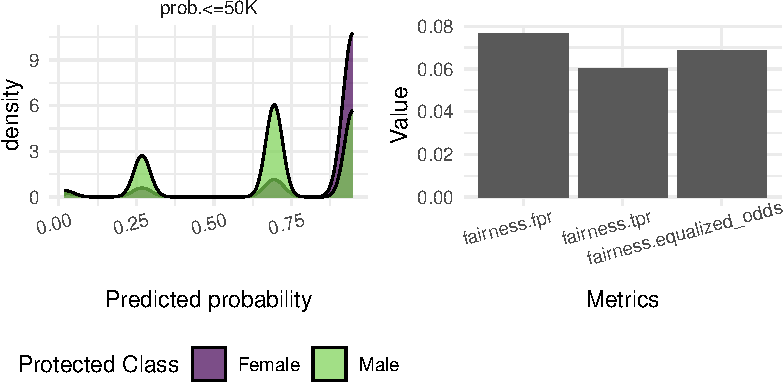
\includegraphics[width=1\textwidth,height=\textheight]{chapters/chapter14/algorithmic_fairness_files/figure-pdf/fig-fairness-1.pdf}

}

\caption{\label{fig-fairness}Fairness prediction density plot (left)
showing the density of predictions for the positive class split by
``Male'' and ``Female'' individuals. The metrics comparison barplot
(right) displays the model's scores across the specified metrics.}

\end{figure}

In this example (Figure~\ref{fig-fairness}), we can see the model is
more likely to predict `Female' observations as having a lower salary.
This could be due to systemic prejudices seen in the data, i.e., women
are more likely to have lower salaries due to societal biases, or could
be due to bias introduced by the algorithm. As the right plot indicates
that all fairness metrics exceed 0.05, this supports the argument that
the algorithm may have introduced further bias (with the same caveat
about the 0.05 threshold).

\hypertarget{fair-machine-learning}{%
\section{Fair Machine Learning}\label{fair-machine-learning}}

If we detect that our model is unfair, then a natural next step is to
mitigate such biases. \texttt{mlr3fairness} comes with several options
to address biases in models, which broadly fall into three categories
(Caton and Haas 2020):

\begin{enumerate}
\def\labelenumi{\arabic{enumi}.}
\tightlist
\item
  Preprocessing\index{preprocessing} data -- The underlying data is
  preprocessed in some way to address bias in the data before it is
  passed to the
  \href{https://mlr3.mlr-org.com/reference/Learner.html}{\texttt{Learner}};
\item
  Employing fair models -- Some algorithms can incorporate fairness
  considerations directly, for example, generalized linear model with
  fairness constraints (\texttt{lrn("classif.fairzlrm")}).
\item
  Postprocessing model predictions -- Heuristics/algorithms are applied
  to the predictions to mitigate biases present in the predictions
\end{enumerate}

All methods often slightly decrease predictive performance and it can
therefore be useful to try all approaches to empirically see which
balance predictive performance and fairness. In general, all biases
should be addressed at their root cause (or as close to it) as possible
as any other intervention will be suboptimal.

Pre- and postprocessing schemes can be integrated using
\href{https://mlr3pipelines.mlr-org.com}{\texttt{mlr3pipelines}}\index{\texttt{mlr3pipelines}}
(Chapter~\ref{sec-pipelines}). We provide two examples below, first
preprocessing to balance observation weights with
\texttt{po("reweighing\_wts")} and second post-processing predictions
using \texttt{po("EOd")}. The latter enforces the equalized odds
fairness definition by stochastically flipping specific predictions. We
also test \texttt{lrn("classif.fairzlrm")} against the other methods.

\begin{Shaded}
\begin{Highlighting}[]
\CommentTok{\# load learners}
\NormalTok{lrn\_rpart }\OtherTok{=} \FunctionTok{lrn}\NormalTok{(}\StringTok{"classif.rpart"}\NormalTok{, }\AttributeTok{predict\_type =} \StringTok{"prob"}\NormalTok{)}
\NormalTok{lrn\_rpart}\SpecialCharTok{$}\NormalTok{id }\OtherTok{=} \StringTok{"rpart"}
\NormalTok{l1 }\OtherTok{=} \FunctionTok{as\_learner}\NormalTok{(}\FunctionTok{po}\NormalTok{(}\StringTok{"reweighing\_wts"}\NormalTok{) }\SpecialCharTok{\%\textgreater{}\textgreater{}\%} \FunctionTok{lrn}\NormalTok{(}\StringTok{"classif.rpart"}\NormalTok{))}
\NormalTok{l1}\SpecialCharTok{$}\NormalTok{id }\OtherTok{=} \StringTok{"reweight"}

\NormalTok{l2 }\OtherTok{=} \FunctionTok{as\_learner}\NormalTok{(}\FunctionTok{po}\NormalTok{(}\StringTok{"learner\_cv"}\NormalTok{, }\FunctionTok{lrn}\NormalTok{(}\StringTok{"classif.rpart"}\NormalTok{)) }\SpecialCharTok{\%\textgreater{}\textgreater{}\%}
  \FunctionTok{po}\NormalTok{(}\StringTok{"EOd"}\NormalTok{))}
\NormalTok{l2}\SpecialCharTok{$}\NormalTok{id }\OtherTok{=} \StringTok{"EOd"}

\CommentTok{\# preprocess by collapsing factors}
\NormalTok{l3 }\OtherTok{=} \FunctionTok{as\_learner}\NormalTok{(}\FunctionTok{po}\NormalTok{(}\StringTok{"collapsefactors"}\NormalTok{) }\SpecialCharTok{\%\textgreater{}\textgreater{}\%} \FunctionTok{lrn}\NormalTok{(}\StringTok{"classif.fairzlrm"}\NormalTok{))}
\NormalTok{l3}\SpecialCharTok{$}\NormalTok{id }\OtherTok{=} \StringTok{"fairzlrm"}

\CommentTok{\# load task and subset by rows and columns}
\NormalTok{task }\OtherTok{=} \FunctionTok{tsk}\NormalTok{(}\StringTok{"adult\_train"}\NormalTok{)}
\NormalTok{task}\SpecialCharTok{$}\FunctionTok{set\_col\_roles}\NormalTok{(}\StringTok{"sex"}\NormalTok{, }\StringTok{"pta"}\NormalTok{)}\SpecialCharTok{$}
  \FunctionTok{filter}\NormalTok{(}\FunctionTok{sample}\NormalTok{(task}\SpecialCharTok{$}\NormalTok{nrow, }\DecValTok{500}\NormalTok{))}\SpecialCharTok{$}
  \FunctionTok{select}\NormalTok{(}\FunctionTok{setdiff}\NormalTok{(task}\SpecialCharTok{$}\NormalTok{feature\_names, }\StringTok{"education\_num"}\NormalTok{))}

\CommentTok{\# run experiment}
\NormalTok{lrns }\OtherTok{=} \FunctionTok{list}\NormalTok{(lrn\_rpart, l1, l2, l3)}
\NormalTok{bmr }\OtherTok{=} \FunctionTok{benchmark}\NormalTok{(}\FunctionTok{benchmark\_grid}\NormalTok{(task, lrns, }\FunctionTok{rsmp}\NormalTok{(}\StringTok{"cv"}\NormalTok{, }\AttributeTok{folds =} \DecValTok{5}\NormalTok{)))}
\NormalTok{meas }\OtherTok{=} \FunctionTok{msrs}\NormalTok{(}\FunctionTok{c}\NormalTok{(}\StringTok{"classif.acc"}\NormalTok{, }\StringTok{"fairness.eod"}\NormalTok{))}
\NormalTok{bmr}\SpecialCharTok{$}\FunctionTok{aggregate}\NormalTok{(meas)[,}
\NormalTok{  .(learner\_id, classif.acc, fairness.equalized\_odds)]}
\end{Highlighting}
\end{Shaded}

\begin{verbatim}
   learner_id classif.acc fairness.equalized_odds
1:      rpart       0.836                  0.1981
2:   reweight       0.828                  0.1860
3:        EOd       0.826                  0.1969
4:   fairzlrm       0.814                  0.1987
\end{verbatim}

We can study the result using built-in plotting functions, below we use
\href{https://mlr3fairness.mlr-org.com/reference/fairness_accuracy_tradeoff.html}{\texttt{fairness\_accuracy\_tradeoff()}},
to compare classification accuracy (default accuracy measure for the
function) and equalized odds (\texttt{msr("fairness.eod")}) across
cross-validation folds.

\begin{Shaded}
\begin{Highlighting}[]
\FunctionTok{fairness\_accuracy\_tradeoff}\NormalTok{(bmr, }\AttributeTok{fairness\_measure =} \FunctionTok{msr}\NormalTok{(}\StringTok{"fairness.eod"}\NormalTok{),}
  \AttributeTok{accuracy\_measure =} \FunctionTok{msr}\NormalTok{(}\StringTok{"classif.ce"}\NormalTok{)) }\SpecialCharTok{+}
\NormalTok{  ggplot2}\SpecialCharTok{::}\FunctionTok{scale\_color\_viridis\_d}\NormalTok{(}\StringTok{"Learner"}\NormalTok{) }\SpecialCharTok{+}
\NormalTok{  ggplot2}\SpecialCharTok{::}\FunctionTok{theme\_minimal}\NormalTok{()}
\end{Highlighting}
\end{Shaded}

\begin{figure}[H]

{\centering 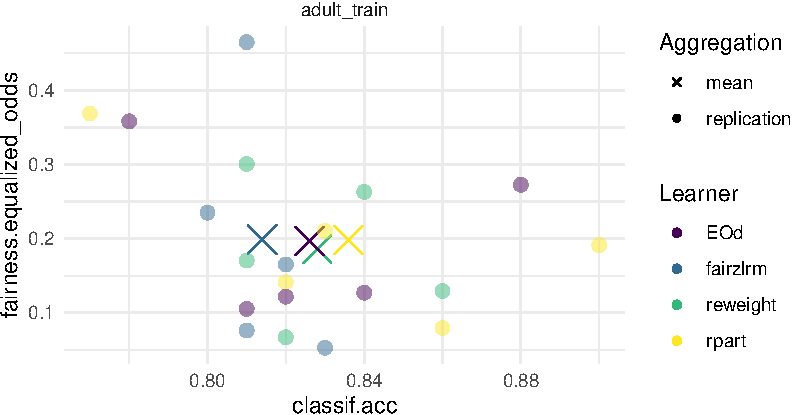
\includegraphics[width=1\textwidth,height=\textheight]{chapters/chapter14/algorithmic_fairness_files/figure-pdf/fig-fairness-tradeoff-1.pdf}

}

\caption{\label{fig-fairness-tradeoff}Comparison of learners with
respect to classification accuracy (x-axis) and equalized odds (y-axis)
across (dots) and aggregated over (crosses) folds.}

\end{figure}

Looking at the table of results and Figure~\ref{fig-fairness-tradeoff},
the reweighting method appears to yield marginally better fairness
metrics than the other methods though the difference is unlikely to be
significant. So in this case, we would likely conclude that introducing
bias mitigation steps did not improve algorithmic fairness.

As well as manually computing and analyzing fairness metrics, one could
also make use of
\href{https://mlr3tuning.mlr-org.com}{\texttt{mlr3tuning}}\index{\texttt{mlr3tuning}}
(Chapter~\ref{sec-optimization}) to automate the process with respect to
one or more metrics (Section~\ref{sec-multi-metrics-tuning}).

\hypertarget{conclusion-11}{%
\section{Conclusion}\label{conclusion-11}}

The functionality introduced above is intended to help users investigate
their models for biases and potentially mitigate them. Fairness metrics
can not be used to prove or guarantee fairness. Deciding whether a model
is fair requires additional investigation, for example, understanding
what the measured quantities represent for an individual in the real
world and what other biases might exist in the data that could lead to
discrepancies in how, for example, covariates or the label are measured.

The simplicity of fairness metrics means they should only be used for
exploratory purposes, and practitioners should not solely rely on them
to make decisions about employing a machine learning model or assessing
whether a system is fair. Instead, practitioners should look beyond the
model and consider the data used for training and the process of data
and label acquisition. To help in this process, it is important to
provide robust documentation for data collection methods, the resulting
data, and the models resulting from this data. Informing auditors about
those aspects of a deployed model can lead to a better assessment of a
model's fairness. Questionnaires for machine learning models and data
sets have been previously proposed in the literature and are available
in
\href{https://mlr3fairness.mlr-org.com}{\texttt{mlr3fairness}}\index{\texttt{mlr3fairness}}
from automated report templates
(\href{https://mlr3fairness.mlr-org.com/reference/report_modelcard.html}{\texttt{report\_modelcard()}}
and
\href{https://mlr3fairness.mlr-org.com/reference/report_datasheet.html}{\texttt{report\_datasheet()}})
using R markdown for data sets and machine learning models. In addition,
\href{https://mlr3fairness.mlr-org.com/reference/report_fairness.html}{\texttt{report\_fairness()}}
provides a template for a fairness
report\index{fairness report}{\marginnote{\begin{footnotesize}Fairness
Report\end{footnotesize}}} inspired by the Aequitas Toolkit (Saleiro et
al. 2018).

We hope that pairing the functionality available in
\texttt{mlr3fairness} with additional exploratory data analysis, a solid
understanding of the societal context in which the decision is made and
integrating additional tools (e.g.~interpretability methods seen in
Chapter~\ref{sec-interpretation}), might help to mitigate or diminish
unfairness in systems deployed in the future.

\hypertarget{tbl-api-fair}{}
\begin{longtable}[]{@{}
  >{\raggedright\arraybackslash}p{(\columnwidth - 4\tabcolsep) * \real{0.3333}}
  >{\raggedright\arraybackslash}p{(\columnwidth - 4\tabcolsep) * \real{0.3333}}
  >{\raggedright\arraybackslash}p{(\columnwidth - 4\tabcolsep) * \real{0.3333}}@{}}
\caption{\label{tbl-api-fair}Important classes and functions covered in
this chapter with underlying class (if applicable), class constructor or
function, and important class fields and methods (if
applicable).}\tabularnewline
\toprule\noalign{}
\begin{minipage}[b]{\linewidth}\raggedright
Class
\end{minipage} & \begin{minipage}[b]{\linewidth}\raggedright
Constructor/Function
\end{minipage} & \begin{minipage}[b]{\linewidth}\raggedright
Fields/Methods
\end{minipage} \\
\midrule\noalign{}
\endfirsthead
\toprule\noalign{}
\begin{minipage}[b]{\linewidth}\raggedright
Class
\end{minipage} & \begin{minipage}[b]{\linewidth}\raggedright
Constructor/Function
\end{minipage} & \begin{minipage}[b]{\linewidth}\raggedright
Fields/Methods
\end{minipage} \\
\midrule\noalign{}
\endhead
\bottomrule\noalign{}
\endlastfoot
\href{https://mlr3fairness.mlr-org.com/reference/MeasureFairness.html}{\texttt{MeasureFairness}}
& \texttt{msr("fairness",\ ...)} & - \\
- &
\href{https://mlr3fairness.mlr-org.com/reference/fairness_prediction_density.html}{\texttt{fairness\_prediction\_density()}}
& \\
- &
\href{https://mlr3fairness.mlr-org.com/reference/compare_metrics.html}{\texttt{compare\_metrics()}}
& - \\
\href{https://mlr3fairness.mlr-org.com/reference/mlr_pipeops_reweighing.html}{\texttt{PipeOpReweighingWeights}}
& \texttt{po("reweighing\_wts")} & - \\
\href{https://mlr3fairness.mlr-org.com/reference/mlr_pipeops_equalized_odds.html}{\texttt{PipeOpEOd}}
& \texttt{po("EOd")} & - \\
- &
\href{https://mlr3fairness.mlr-org.com/reference/fairness_accuracy_tradeoff.html}{\texttt{fairness\_accuracy\_tradeoff()}}
& \\
- &
\href{https://mlr3fairness.mlr-org.com/reference/report_fairness.html}{\texttt{report\_fairness()}}
& - \\
\end{longtable}

\hypertarget{exercises-12}{%
\section{Exercises}\label{exercises-12}}

\begin{enumerate}
\def\labelenumi{\arabic{enumi}.}
\tightlist
\item
  Train a model of your choice on \texttt{tsk("adult\_train")} and test
  it on \texttt{tsk("adult\_test")}, use any measure of your choice to
  evaluate your predictions. Assume our goal is to achieve parity in
  false omission rates across the protected `sex' attribute. Construct a
  fairness metric that encodes this and evaluate your model. To get a
  deeper understanding, look at the
  \href{https://mlr3fairness.mlr-org.com/reference/groupwise_metrics.html}{\texttt{groupwise\_metrics}}
  function to obtain performance in each group.
\item
  Improve your model by employing pipelines that use pre- or
  post-processing methods for fairness. Evaluate your model along the
  two metrics and visualize the resulting metrics. Compare the different
  models using an appropriate visualization.
\item
  Add ``race'' as a second sensitive attribute to your dataset. Add the
  information to your task and evaluate the initial model again. What
  changes? Again study the \texttt{groupwise\_metrics}.
\item
  In this chapter we were unable to reduce bias in our experiment. Using
  everything you have learned in this book, see if you can successfully
  reduce bias in your model. Critically reflect on this exercise, why
  might this be a bad idea?
\end{enumerate}

\bookmarksetup{startatroot}